\subsection{Versuchsaufbau}
\label{sec:Versuchsaufbau}

Der verwendete Aufbau ist in Abbildung~\ref{fig: aufbau} dargestellt. Alle Bauteile sind auf einer Schiene angebracht, sodass die
relativen Abstände variiert werden können. Bevor relevante Merkmale des Lasers vermessen werden können, ist eine
Justage des Aufbaus notwendig. Hierzu wird ein weiterer Laser und zwei Beugungsblenden verwendet. Am Laserrohr wird eine Hochspanung
angelegt, die die notwendige Gasentladung hervorruft. Durch Justierschrauben an den konfokalen Resonatorspiegeln (Radius jeweils $\SI{1.4}{\meter}$)
und dem Laserrohr werden die Elemente so eingestellt, dass die optischen Achsen aufeinander liegen und der Laser anfängt zu leuchten.
Zur Intensitätsmessung wird eine Photodiode verwendet, die hinter dem Laser positioniert ist.
%\begin{figure}
%  \centering
%  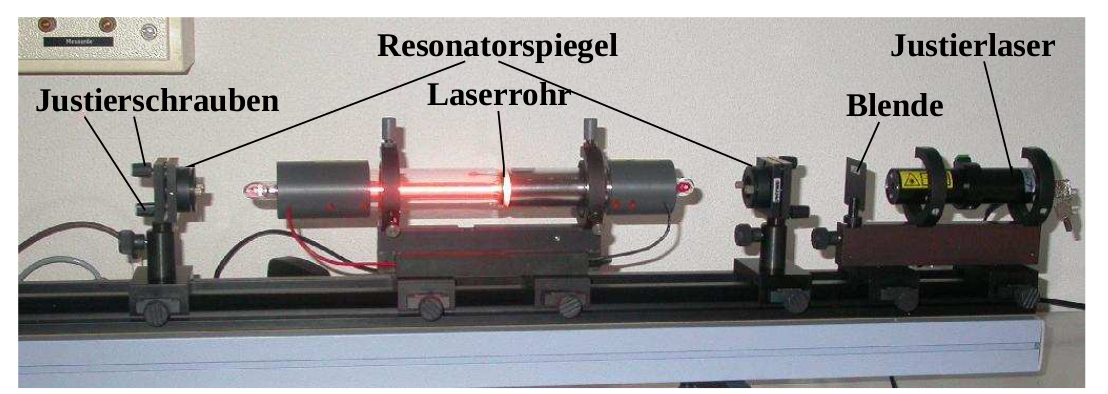
\includegraphics[width=0.75\columnwidth]{pictures/aufbau.png}
%  \caption{\cite{Anleitung}}
%  \label{fig:aufbau}
%\end{figure}
